\documentclass[
	letterpaper, % Paper size, specify a4paper (A4) or letterpaper (US letter)
	10pt, % Default font size, specify 10pt, 11pt or 12pt
]{CSUniSchoolLabReport}

\usepackage{fancyvrb}

% redefine \VerbatimInput
\RecustomVerbatimCommand{\VerbatimInput}{VerbatimInput}%
{fontsize=\footnotesize,
 %
 frame=lines,  % top and bottom rule only
 framesep=2em, % separation between frame and text
 rulecolor=\color{Gray},
 %
 label=\fbox{\color{Black} Power Flow Solution — Base Case}, 
 labelposition=topline,
 %
 commandchars=\|\(\), % escape character and argument delimiters for
                      % commands within the verbatim
 commentchar=*        % comment character
}

%----------------------------------------------------------------------------------------
%	REPORT INFORMATION
%----------------------------------------------------------------------------------------

\title{Lab Six (Part A)\\ Power Systems Analysis \\ EECE5682} % Report title

\author{Michael \textsc{Brodskiy}\\ \small \href{mailto:Brodskiy.M@Northeastern.edu}{Brodskiy.M@Northeastern.edu}}

\date{November 17, 2024} % Date of the report

%----------------------------------------------------------------------------------------


\begin{document}

\maketitle % Insert the title, author and date using the information specified above

\begin{center}
	\begin{tabular}{l r}
		Date Performed: & \today \\ % Date the experiment was performed
		Instructor: & Professor \textsc{Abur} \\ % Instructor/supervisor
	\end{tabular}
\end{center}

\newpage

\begin{abstract}

  This laboratory experiment allows the user to explore power flow solutions to a real-life instance of a 30-bus system. Furthermore, by performing the experiment, the individual will develop a better understanding of total transfer capability (TTC) between buses, and how this can be improved.

\end{abstract}

\begin{flushleft}

  \textsc{Keywords:} \underline{power flow}, \underline{30-bus system}, \underline{total transfer capability}

\end{flushleft}

\newpage

\section{Introduction \& Objectives}

We begin by constructing the provided 30-bus system in the Power Education Toolbox (PET) program. The system looks as follows:

\begin{figure}[H]
  \centering
  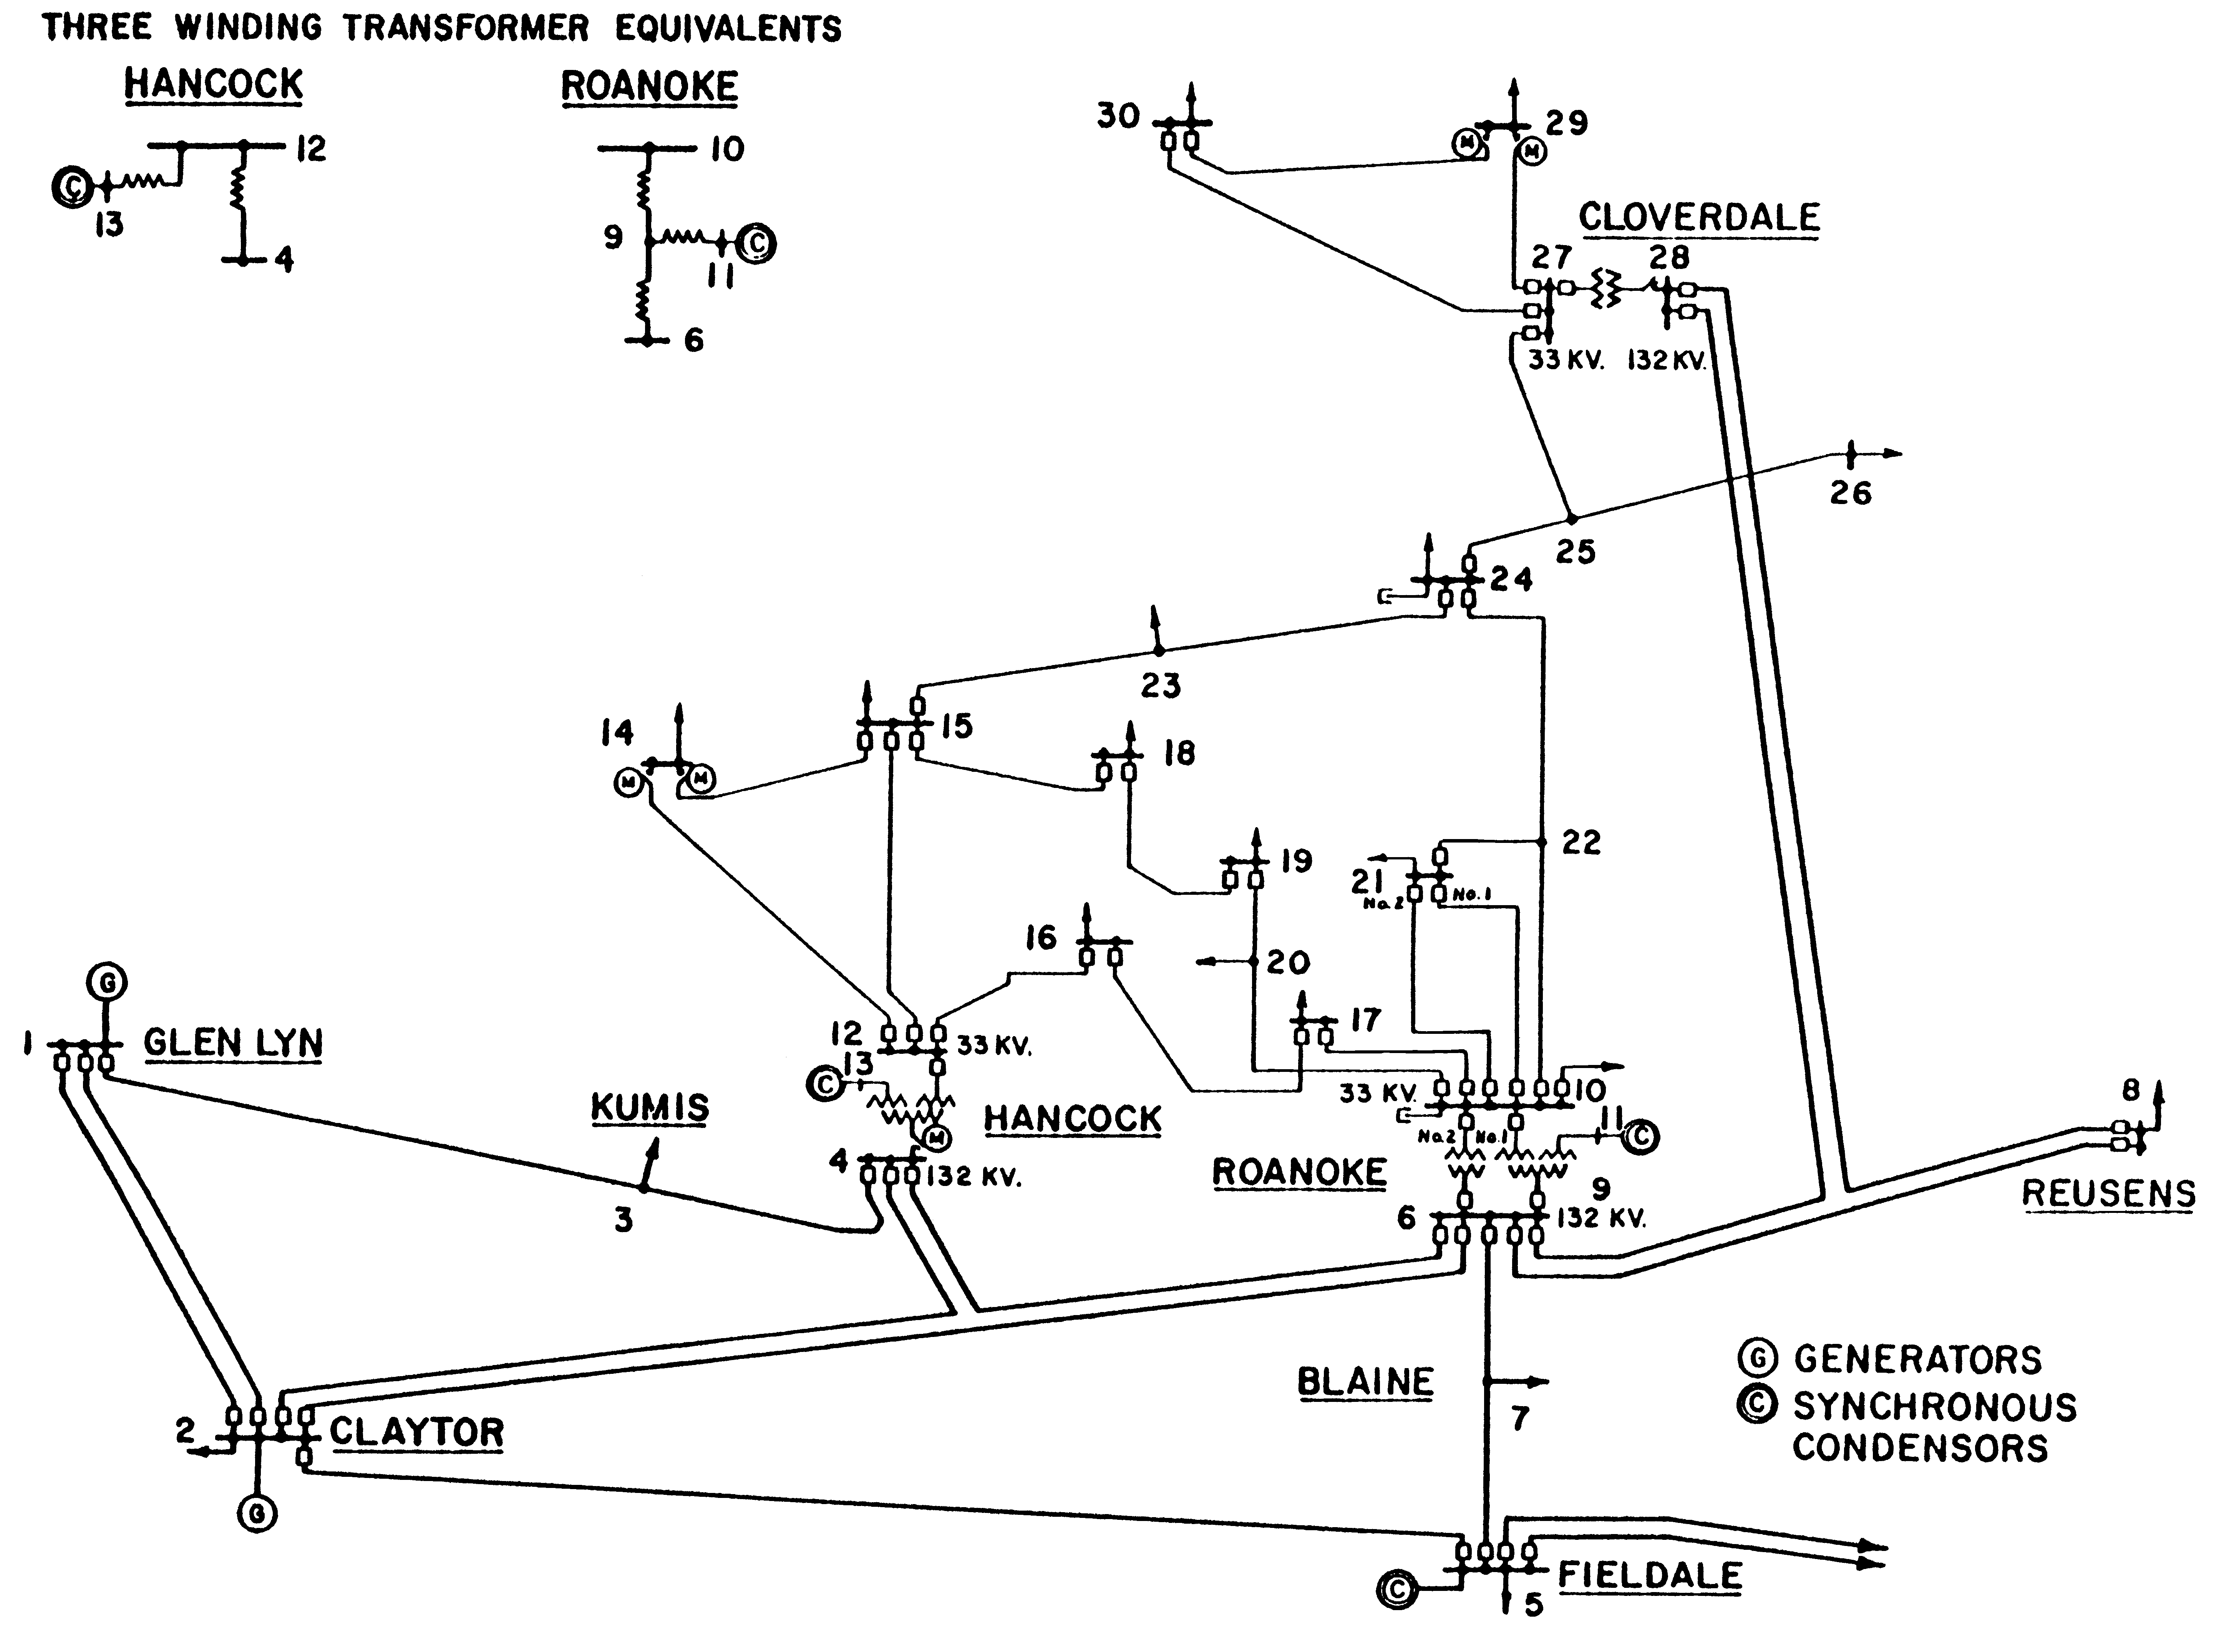
\includegraphics[width=.9\textwidth]{Figures/Lab\ Six/30bus600}
  \caption{The 30-Bus System}
  \label{fig:1}
\end{figure}

\section{Experimentation}

\subsection{Part 1}

We may run the base case solution to get:

\VerbatimInput{Figures/LabSix/PFOutPartA.dat}

\subsection{Part 2}

We may determine the total transfer capability (TTC) from the source (bus 1) to the sink (bus 25) by slowly increasing the real power load of the sink. Taking steps of $5[\si{\mega\watt}]$, we begin increasing from 0. We may observe that the solution diverges when we change the real load to $80[\si{\mega\watt}]$. We reduce by $1[\si{\mega\watt}]$ until we get a real solution. This occurs at $P_L=75[\si{\mega\watt}]$. As such, we have determined that the TTC is $75[\si{\mega\watt}]$.

\subsection{Part 3}

Using the result from Part 2, we run a simulation with $P_L=75[\si{\mega\watt}]$ for the sink. This gives us the following data:

\VerbatimInput[label=Power Flow Solution — TTC Case]{Figures/LabSix/PFOutPartC.dat}

\subsection{Part 4}

With the added shunt capacitor at bus 26, we now have a new TTC solution. We repeat the process outline in Part 2 to obtain a new TTC solution of $P_L=82[\si{\mega\watt}]$. Running the power flow solution gets us:

\VerbatimInput[label=Power Flow Solution — TTC Case w/Added Capacitor]{Figures/LabSix/PFOutPartD.dat}

\subsection{Part 5}

Finally, we want to add $5[\si{\mega\watt}]$ to the TTC determined in Part 4. We may observe that the added shunt capacitance increased the TTC. Thus, we may conclude that increasing the susceptance may improve the TTC. Slowly increasing the susceptance by $.01[p.u.]$, we determine that a valid way to increase the TTC by $5[\si{\mega\watt}]$ (from $82\to87[\si{\mega\watt}]$) is to change the susceptance from $.2\to.34[p.u.]$. This gets us the following solution:

\VerbatimInput[label=Power Flow Solution — TTC Increased by 5]{Figures/LabSix/PFOutPartE.dat}

Note that we could have also added a capacitor to bus 25 itself to increase the value.

\end{document}
